%% Thesis Introduction --------------------------------------------------
\chapter{Introduction} 

Computer network technologies in the recent years have become the predominant
communication medium of our digital era.  In 2011, a third of the global
population is Internet-connected through a wide range of network
technologies~\cite{itufacts2011}, while Internet resources, based on
estimations, generate 3.4\% of the global GDP~\cite{duRausas:2011un}. In
parallel, a large fraction of our everyday social life depends on network
connectivity (e.g.~Social networking, e-mail, e-shopping etc.). Due to the
increasing importance of network technologies, functional requirements are
constantly evolving and network infrastructures {\emph must} be future-proof
against increasing traffic rates and performance and security policy complexity.

From an architectural point of view, network functionality is logically
separated in two planes: the control and data plane. The data plane is
responsible to forward rapidly packets between device ports.  The control plane
is responsible to orchestrate and transform network policy inputs (e.g.~device
configuration, routing protocol etc.) into efficient forwarding policies for the
data plane. The performance of a network relies on the performance of both
planes of functionality. Recent efforts in ASIC design~\cite{covington13}, for
hardware-based forwarding devices, and network IO
performance~\cite{routebricks,rizzo12,Han10}, for software-based switches,
provide strong evidence on the scalability of the data plane functionality in
supporting current network speeds.  In contrast, existing control plane
architectures face significant limitations to match the evolution of the data
plane from a performance perspective~(Section~\ref{sec:background:netcontrol}). 

% Current data plane functionality experiences a significant evolutionary mismatch
% in comparison to the data plane. 
In contrast to the device data plane performance, which can been described
through the forwarding rate and processing latency of the device, control plane
performance definition has a much higher dimensionality and is tightly coupled
with the deployment environment. An example of a significant performance
parameter of the control plane is the responsiveness of the control plane. Data
plane routing and link layer loop avoidance algorithms use decentralised
consensus algorithms to share network state and achieve resilient and
distributed control.  Due to the distributed nature of existing control
algorithms, the convergence time during state changes is on average orders of
magnitude higher in comparison to the packet processing latency of the data
plane. This latency difference becomes important for high capacity links, as
the number of packets forwarded over an under-optimal path, after a change in
network connectivity, is increased.  Similarly, a significant performance parameter
for the control plane of a network is functional evolvability.  Existing control
plane functionality is distributed and integrated with the network device, thus
requiring significant network-wide device upgrades in order to evolve the
control plane.  In addition, control plane performance definition involves
subjective non-measurable parameters, such as user friendliness.  Current
network control plane architectures expose a highly complex control abstraction
to the user, in order to fulfil the requirements for generic and universally
applicable control, which fail to scale from a management
perspective~\cite{Mahajan02}.

The recent introduction of the Software Defined Network (SDN) paradigm defines a
novel unified control abstraction for network devices which enables higher
flexibility to redefine the control plane logic and scale
performance~(Section~\ref{sec:background:sdn}).  The SDN paradigm supports a
wide range of control mechanisms, and can be used to synthesize rapidly novel
high-level control abstraction.  In this dissertation we argue the thesis that: 

\begin{quotation} 
  Current network technologies face a significant and multi-dimensional
  performance bottleneck on the control plane of the network. In order to
  improve control plane performance in a scalable manner we must redesign the
  control plane functionality, using the SDN control abstraction, in order to
  optimize specific aspects and match the deployment environment requirements. 
\end{quotation}

% As a result of the elevated role of the
% network abstraction, the functional requirements of a modern network have
% significantly evolved in the recent years and some network functionalities face
% scalability problems. In parallel, the strong requirement for backwards
% compatibility keeps core Internet protocols unchanged since the 70's, unable to
% address these scalability problems by design.  As a result, current network
% technologies are not able to fulfil the novel functional requirements of the
% technological and social setting and clean slate re-design of the Internet to
% fulfil these requirements is not possible.

% While computer networks play an important role in our everyday life, their
% strong backwards compatibility requirement create a important gap in their
% functionality evolution in order to fulfil current evolving communication
% needs.

% Our work focuses on the scalability problem of modern networks and examines
% whether evolved network control logic, designed for specific network
% environments, can scale network functionality. In this dissertation we argue the
% thesis that: 
% 
% \begin{quotation} 
%   Computer network design can scale specific functional aspects through
%   context-aware evolved control planes.  Such control mechanisms should address
%   the requirements of the deployment environment and establish new
%   domain-specific control abstractions that take advantage of its distinct
%   properties. 
% \end{quotation}

For the remainder of this introduction chapter we justify the importance of this
thesis.  In Section~\ref{sec:intro:motivations} we discuss the evolution of
existing network technologies and the scalability limitations incurred by
existing control plane functionality. In Section~\ref{sec:intro:contributions},
we list our contributions and in Section~\ref{sec:intro:outline}, we present the
content of each chapter of the thesis.

\section{Motivation} \label{sec:intro:motivations}

In this section we discuss some of the motivations for our thesis. Specifically,
we present the evolutionary aspect of network technologies, in terms of
requirements, applications and connection technologies
(Section~\ref{sec:intro:net_evolution}) and highlight some of the limitation of
the current control plane
technologies~(Section~\ref{sec:intro:control_limitations}).

\subsubsection*{Computer network growth} \label{sec:intro:net_evolution}

\begin{figure}[ht] 
  \centering 
  \subfigure[global Internet traffic
  trend]{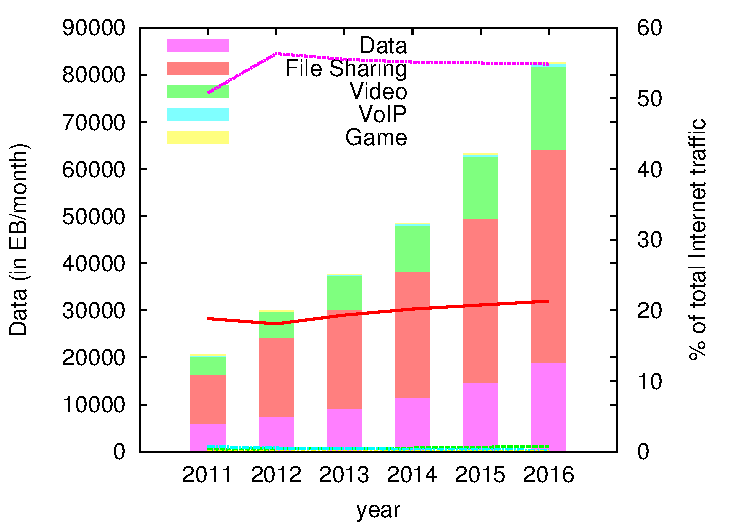
\includegraphics[width=0.48\textwidth]{Introduction/IntroductionFigs/internet} \label{fig:mobile} }
  \subfigure[global mobile Internet traffic
  trend]{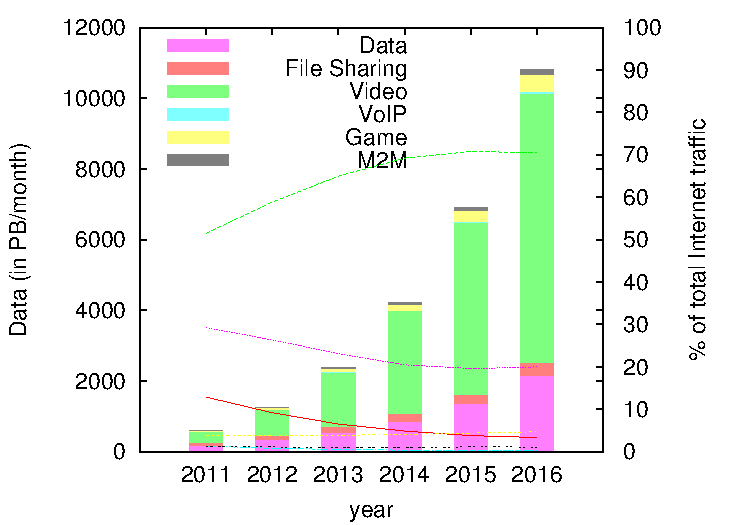
\includegraphics[width=0.48\textwidth]{Introduction/IntroductionFigs/mobile} \label{fig:internet} }
  \caption{Cisco Visual Network Index reports on global network traffic per
    application for Internet (Figure~\ref{fig:internet}) and for Mobile
    Internet (Figure~\ref{fig:mobile}). Application } 
  \label{fig:internet_applications} 
\end{figure}

\begin{table} 
  \centering
  {\tiny
    \begin{tabular}{ | p{3cm} | c c c c | } 
      \hline
      Application                              & rate                        & latency        & jitter         & \# connections \\ \hline 
      web~\cite{Akamai_4_seconds,Butkiewicz11} & no requirement              & $<$ 4 sec        & no requirement & $>$ 10 (median) \\ 
      video~\cite{Finamore11}                  & 0.3~(240p) - 5~(1080p) Mbps & no requirement & -              &  1 \\ 
      peer-to-peer~\cite{Rasti07,pouwelse2004} & maximum possible            & no requirement & no requirement &  maximum possible \\ 
      VoIP                                     & 100 kbps~(voice) - 1.5 Mbps~(voice and HD video)    & $<$ 500 msec       & $<$ 100msec      & 1 \\ 
      gaming~\cite{armitage2006networking}     &  $<$ 100 kbps                 & $<$ 100 msec       & $<$ 50 msec      & 1\\ \hline
    \end{tabular} 
  }
  \caption{Network performance requirements for a set of popular traffic classes.} 
  \label{tbl:application_requirement}
\end{table}

% A core building block of computer networks is the idea of packet-switched
% networks~\cite{Licklider1963}.  In comparison to the popular circuit-switched
% network technologies of the past, packet-switched networks increase
% the medium utilisation and provide strong resilience to
% link losses.  Packet-switched networks achieve higher medium utilisation by
% delivery guarantees relaxation and data transmission multiplexing, while data
% propagation can dynamically modify end-to-end paths, if a path becomes unavailable. 

% a historical perspective on computer networks 
One of the key mechanisms that formed the objective conditions for the digital
revolution of our era, was the concept of computer networking.  Computer
networking refers to the ability of two computers to exchange data over a
communication medium. A first attempt to implement a computer network of
significant size was the {\it ARPANET} \/system, a novel communication system of
the times which provided higher resilience and performance in comparison to
existing circuit-switched communication systems.  ARPANET~\cite{beranek81} was
adopted by a small number of US education and research institutes and allowed,
for the first time in computing history, to interconnect multiple mainframes
over a mess network. The initial set of standardised applications provided
elementary mechanisms to exchange data: e-mail~\cite{RFC0561},
FTP~\cite{RFC0354} and voice~\cite{RFC0741}. ARPANET was later replaced by the
NSFNET~\cite{Mills:1987tt} in the 80's, which finally evolved in today's
Internet.  As part of this transition, the research community developed also the
standards for the Internet protocol suite~\cite{Clark:1988}.

Although the concept of computer networks was conceived in the 1960's,
approximately 20 years since the implementation of a programmable computer, the
adoption, as well as, the development of the technology was radical over the
years. Computer networks have managed to provide a sufficient abstraction to
replace a number of traditional communication systems (e.g.~Telephone networks)
and support the requirements for a wide spectrum of applications and deployment
environments. Since the ARPANET time, computer networks gained a significant
position in the global social apparatus, driven by two major adopters: {\it personal
  computing users} and {\it businesses}.

% why computer networking is successful from the user perspective
For personal computer users, network technologies provide the medium to access
rich informations sources and interconnect users and devices seamlessly. An
end-user nowadays can easily use his personal computer, when connected to an
Internet gateway, to connect to system abstractions like the World Wide Web (WWW)
and the Cloud, and access a wealth of information and services.  Currently,
the WWW is the ultimate information source of our times, providing free access
to a large portion of the global human knowledge, while the Web 2.0
functionality of the modern Web enables the development of highly responsive
services which replace traditional information distribution
mechanisms~\cite{stempel2000}.  Recent development in network applications have
established novel mechanisms for fast and wide-scale social interaction.
Currently, Online Social Networks (OSN) interconnect millions of users across
the world, while instant messaging services, like google chat and Skype, enable
real-time text, voice and video communication over the Internet.  In addition,
the radical reduction in cost and size of network-enabled personal computers, as
modelled by Moore's Law, has increased significantly the number of devices
per-user and subsequently increase the network connectivity requirements.  More
and more devices are shipped with network support and 
requires connectivity. The constantly increasing adoption of network
technologies by person computer users fuels a significant portion of network
innovation and motivates the development of new connection mechanisms (e.g.
mobile Internet).  The important role of computer networks for users can be
further reflected in the government level debate to proclaim Internet
connectivity as a fundamental human right~\cite{klang2005human, Wicker2013},
introducing significant technological challenges to scale Internet connectivity
for the global population~\cite{cerf2012}.

% why computer become important for the global economy too? 

% The business sector adopters employ computer networking technologies to
% establish a reliable business service middleware and a scalable, fast and
% low-cost channel to reach costumers. The importance of network technologies for
% the business world can be reflected on the value that the Internet generates,
% which is computed to be 4,3\% of the global GDP\@.  
Computer network technologies and infrastructures have become a valuable asset
for the business sector as well. Business sector adopters employ computer
networks primarily as a cheap, fast and multi-functional communication medium to
interconnect business logic and distribute content to users. The success of
network technologies to provide these functionalities motivates the business
sector to invest in the technology, as well as, innovates the usage of the
technologies in new domains~(e.g.~cloud computing abstractions in a data center
and distributed content distribution). Such novel network concepts stress the
capabilities of available connectivity mechanisms, highlighting interesting
scalability problems~(e.g.~large scale data centers face significant problems to
scale layer 2 connectivity).  The increase in the adoption of network
technologies in the business sector can be further identified in the increase of
the number of Internet Autonomous Systems (AS).  Since 1995 the number has
exponentially increased from 2000 ASes to approximately 45000 ASes, reflecting
the increase in the number of organisations using the global Internet
infrastructure as a core communication mechanism for their
business~\cite{potaroo}. This increase in ASes introduced a significant
scalability problems for the control plane of the largest network in the world,
the Internet~\cite{bgp_instab_labovitz:1997}. 

% Network technology penetration is  further augmented in the business sector
% through the cloud abstraction. Multiple businesses use cloud services to
% reduce IT costs and offload infrastructure maintenance to 3rd party providers.

% Computer networks technologies provide the medium to run 
% online shops and content distribution services, the fabric to interconnect big-data 
% processing frameworks and the 

% In order to bridge user experience between its devices new network applications
% have been developed to addresses the user requirement for device interconnection
% and new network paradigms are introduced to enable ubiquitous Internet access to
% the whole range of personal computing devices, like home networks and mobile
% Internet. 

% what about the application requirements
% \paragraph{computer network application dynamics}

The wide adoption of network technologies drives a continuous application
innovation and new network use-cases emerge constantly.  This innovation in
network applications has a significant impact on the complexity of computer
network management.  The two aforementioned general classes of adopters use the
same network technologies to fulfil a diverse set of requirements.  In order to
exemplify this problem, we present in Table~\ref{tbl:application_requirement}
the resource requirements for a number of popular network applications, namely
web traffic, video streaming, peer-to-peer applications,  VoIP and
gaming\todo{tail at scale, add requirements for cloud service providers for map
  reduced applications}. In the table we report the requirements for each
application in terms of bandwidth, latency, jitter and number of connections.
From the table entries, we note that some application pairs have contradicting
requirements, when using a congested link.  For example, peer-to-peer
applications will try to maximize used network capacity, by flooding network
links, and create increase latency and jitter for delay-sensitive
applications like VoIP\@.  These contradictions are further magnified by the
design abstraction of current network protocols, which hides the state of the
lower layers of the network, lucks performance-related semantics and effectively
reduces the short-term effectiveness of end-to-end resource control.  Nowadays,
the importance of the network control plane in network resource management is
increased. During congestion incidents, the control plane must be able to react
at flow-level timescales and dynamically allocate resources to fulfil
application requirements. 

% Computer networking depends to a great extend on the abstraction
% design pattern in order to support scalability and heterogeneity.  The
% abstraction principle is based to a great extend on the OSI
% model~\cite{Day:1983vy}, which tries to separate network functionality into a
% number of layers and define the intermediate interfaces. A side effect
% of this design approach, application developers remain agnostic to lower layer
% internal state.  Further, The OSI model and the TCP/IP protocol suite luck
% performance-related semantics in their interface definitions.  Applications on
% the other hand, tend to behave egotistically and aggressively try to fulfil
% performance requirements in the network environment. As a result, short-scale
% resource allocation in a network becomes difficult due to the diverse nature of
% network applications. In order to exemplify the problem, we list in
% Table~\ref{tbl:application_requirement} a number of key traffic properties for
% popular traffic classes of the Internet. Network applications have diverse
% properties which becomes difficult to address as link utilisation increases. 

% How computer application mix looks in the wire? 
Application innovation complicates also long-term network planning and
introduces a flexibility requirements in the control plane.  In
Figure~\ref{fig:internet_applications}, we plot the estimated traffic volumes
for six popular network application classes between the years 2011-2016 for
mobile and fixed Internet, using data from the Cisco visualization
index~\cite{Mobile:2012vd,Cisco:2012wu}. From the figure, we note that network
traffic is expected to increase an order of magnitude for mobile Internet, while
the fixed Internet traffic is expected to increase four times. The graphs also
point out the short-term application popularity churn.  The video streaming
class is expected to increase significantly both in traffic volume and overall
traffic over the data and file sharing classes, introducing strict requirements
in term of path capacity and latency.  Experience in network application
evolution determines that new network applications are common to gain rapid
popularity, once they are introduced to the users.  Network technologies must
exhibit flexibility and provide a friendly network environment to fulfil the
resource requirement of the new application without infrastructural upgrades.
Furthermore, once network applications establish their popularity between users,
they will maintain a fixed network traffic volume for a long period of time,
depending on the popularity and novelty of the application. The share of the
application traffic with respect to the overall traffic volume of the network
may reduce over time, especially as link speeds increase and new popular
application emerge, but the network should be able to continue providing a
friendly environment for the application for a long period of time.  This
results in a continuous enlargement of the resource allocation policies and
introduces significant complexity on the network control plane.

\todo{review the data of the application trends}
% % How does the network look like in terms of point to point connectivity. 
A significant evolution in network technologies is also observed in the lower
layers of the network abstraction, which encapsulate significant heterogeneity.
Ethernet has been the predominant Internet link layer protocol since the 80's,
mainly due to its low cost and complexity design principle. The network
community has defined standards to run Ethernet over a wide range of medium
types, like coper, fibber, off-licence radio frequencies, satellite links and
mobile networks, while keeping the network abstraction unmodified. This approach
encapsulates a number of medium properties (e.g.~link layer ARQ, link rate),
within the Ethernet abstraction and hides significant performance
characteristics of the lower layer.

% An example of this
% property is the Internet. Internet exhibits a 3 layer hierarchy of ASes, which
% provide scalability and low average path lengths.  Tier 1 and 2 ISPs provide
% forwarding in an homogeneous and fast manner. Such ISP's are in charge of a
% relatively small number of network points and thus are able to upgrade network
% infrastructure with relatively low costs, which can further be offloaded to
% clients through SLA agreements. For Tier-3 ISPs things are a lot different. This
% class of ISPs covers a wide range of services. Also because this is the last hop
% to end users, such networks tend to be large and spread over large geographic
% distances. For this type of networks, connectivity properties are variable,
% users SLA have minimum guarantees, performance depends on the link sharing ratio
% and the medium types. Additionally, the cost to upgrade such networks is high,
% while strong market competition makes difficult to offload costs directly to
% users. A number of measurement studies have described these
% differences~\cite{Huang:2010wb,Dischinger:2007bg}. 

\subsubsection*{Control plane limitations}
\label{sec:intro:control_limitations}

% how does computer networks look like, How the Internet looks like?
% Over the previous section we described the heterogeneity of current computer
% networks and the dynamics of network applications. In order to address these
% properties in an efficient way, computer network technologies should be able to
% evolve. But within existing network systems it is difficult to deploy new
% technologies. 

% Although computer networks are highly important for society the adaptability of
% network technologies to user requirement has not been equal over the years. This
% mismatch can be ascribed to a number of reasons. 

% network design were developed in an environment that had different properties
Unlike traditional distributed systems, the design of network technologies and
protocols must be able to accommodate all potential future requirements. This
fundamental design goals stem both because of the large number of individual
components forming the network, as well
as, the capability of individual components to accommodate protocol
updates~(e.g. ASIC silicons are optimized to implement specific network
functionality at line rate, but they are unable to modify their functionality).
Current control and data plane protocols, unfortunately,  experience a
number of design limitations primarily due to the inability of their designers
to predict the radical adoption of the technology. 
% Existing network technologies experience 
% a mismatch between the functional
% requirements of the environment that they were initially designed for and the
% current network requirements.  
The early adopters of the NSFNET, which defined the Internet protocol standards,
were universities and research facilities and the design process aimed to
provide support for asynchronous communication applications, low link speeds and
best-effort connectivity guarantees. Furthermore, in order to ease the design of
network devices, the protocols followed the end-to-end design
principle~\cite{end2endIP}. The control plane on the intermediate hops of the
path ensures long-term network connectivity.  Current Internet protocols have
managed to provide a strongly connected network, but as network size and
complexity increases, the control plane becomes an important mechanism to
optimize network performance.
% ~\todo{ratio of transmission to propagation delay is reduced}.  

The existing Internet protocols were selected through a ``natural selection
process'' against other isomorphic protocols, developed during the early days of
the NSFNET\@. During that period, the OSI and ITU organisations published a
number of network protocol definitions~\cite{x.213,x.233} which provided
connectivity for all layers of the network abstraction, while the ATM Forum also
defined similar higher-layer protocols, on top of the ATM
technology~\cite{Siu95}. These protocol attempts provided highly detailed
abstractions, as well as, highly complex protocols which, although, can address
some of the current functional limitations.  Nonetheless, their increased
complexity introduced performance scalability problems for the computational
resources of the time and the protocols became obsolete in favor of current
Internet protocols.

% In the recent years, the limitations of existing network control plane
% mechanisms have become apparent, as a number of fundamental system assumptions
% have changed. 
For the rest of the section, we discuss some important network
limitations of current technologies.

\subparagraph*{Security} 

The initial security requirements for computer network technologies were
minimal. On one hand, early technology adopters, such as educational and
research institutes, used networks to provide open, free and accessible
services, aiming to augment technology adoption. As a result, their security
requirements were minimal. On the other hand, the computing resources of the
time were limited and couldn't support the computation requirements for a
security-aware network design.  In parallel the US Department of Defence~(DoD) ,
in order to ensure secure transmission of classified information, designed and
implemented a number of high security networks, namely MILNET, SIPRnet and
NIPRnet. These networks function as partially stand-alone inter-networks owned
by the DoD and provide strong security primitives in the network design.  Their
design supports low bandwidth connectivity~(primarily HTTP and mail services)
and uses enhanced security mechanisms in the lower layers of the stack along
with existing Internet protocol in the higher layers of the
network~\cite{siprnet}. 

These initial network security requirements are currently invalidated. A McAfee
report from 2009 estimates the cost for cybersecurity to approximately 600
million dollars~\cite{kanan2009unsecured}.  Similarly, during the wikileaks
scandal in 2011~\cite{cablegate}, a significant number of US state documents was
intercepted from the SIPRnet system, exposing the limitation in the design of
the network.  The threat model for network systems is wide and contains numerous
attacks; from information interception to denial-of-service attacks.  
The research community has proposed a number of protocols to address the
security requirements of today network environment, e.g.~IPSEC~\cite{RFC2401}
and loose source routing~\cite{Argyraki09}.  Nonetheless, although such
protocol introduce enhanced security guarantees for the data plane, they also
introduce significant complexity on the control plane of the network. For
example, for IPsec the data plane can implement at line rate the
encryption/decryption task, but an IPsec gateway must maintain protocol state
for each tunnel.  Network security requires security-aware control logic
spanning from the lowest layers of the network abstraction and spread across
the network. 

% \subparagraph*{Network Addressing} 
% When the IP protocol was firstly deployed in the Internet, the size of the
% network was sufficiently small. Host addresses use a 32-bit
% integer, split in byte aligned classes in order to permit aggregation at
% the forwarding entities. Within 10 years, the initial assumptions over the size
% of classes was re-established through the classless Inter-domain routing (CIDR),
% in order to allow better utilisation of the IP space. Within 15 years
% the initial assumption over the size of the address space proved also
% short-sighted, as IP addresses were not sufficient to cover the needs of hosts.  A
% number of layer violations, like NATs, were widely used within the subsequent
% years in order to provide connectivity to the increasing number of end-hosts. In
% order to address this problem within the design of the network protocol, a
% revised version of IP has been proposed~\cite{RFC2460} since 1998, but its
% deployment is slow, as the size of the current Internet makes it extremely
% difficult to replace IPv4 without significant connectivity problems and costs.

\subparagraph*{Network management scalability}

A significant control plane scalability bottleneck can be traced back to the
policy expression interface of current technologies. In
Section~\ref{sec:background:forwarding} we provide an extensive presentation of
the basic network control mechanisms and describe the exposed control
abstraction.  Current network control schemes rely on network administrators to
manually transform the global control policy into localised policies for each
network device. In addition, the layered nature of existing network devices
requires individual configuration for each network layer.  Furthermore, there is
a luck of mechanisms to evaluate the effectiveness and validity of the resulting
network configuration.  Policy evaluation relies on traditional connectivity
testing tools, like ping and tcpdump, and byte and packet SNMP counters from
network devices.  As a result, large-scale network management is a highly
laborious process and requires significant experience. Ultimately, modern
network management interfaces have a significant non-scalable bottleneck on the
``mechanism'' translating the network functional requirement into distributed
device configuration, the network manager.  

% Depending on the device type and role (Router, Firewall,
% Switch), the policy evolution is different and influenced by the structure of
% the network.  

% The unscalable nature of network configuration mechanisms is also reflected on
% the network administrator availability.  

In~\cite{Kim11}. the authors conduct a measurement study on the evolution of the
configuration of two medium-sized campus networks. Their longitude analysis
highlights the constant expansion of the network policy for the two networks, as
well as, the mixture in the network configuration of security and forwarding
control.  In addition, the network configuration process is highly subjective
and depends on the device type and the deployment environment.  Especially for
switch and router configuration, every network policy change translates into a
number of device policy updates across the network, highlighting the restricted
expressiveness of the policy definition languages.  Finally, device policies
over time are common to contain stale rules in order to avoid potential network
misconfiguration, which are pruned only when they are contradicting newer policy
updates or during major policy revisions.  Similarly, in~\cite{Mahajan02} the
authors study global BGP protocol errors and report a significant portion of
protocol misconfiguration which reduce connectivity and performance. These
misconfigurations can be ascribed to the counter intuitive control abstraction
of the routing protocol.  The mismatch between human understanding and network
abstraction is further exemplified in the domain of home networking.
In~\cite{grinter05}, the authors contact a small scale user study and highlight
the mismatch between the user-perceived network connectivity abstraction and the
real network functionality. This mismatch leads to under-optimized network
configuration. Ultimately, homeowners tend to sacrifice security and
performance, in order to reduce the burden of network management. 

The management problem is further augmented by the standalone functionality of
the control plane of a set of common network devices, like performance-enhancing
middleboxes, firewalls and NATs. Such devices maintain a local static network
configuration, disconnected from the distributed control plane of traditional
network devices.  This luck of interaction may introduce unexpected network
behaviours during significant network changes, e.g.~subnetwork disconnections
and reduced host connectivity.  The network management domain requires a
technological revolution, similar to the revolution of high-level programming
language in the 70's.  In order to scale network management performance, we
require new user-friendly control abstractions which can automate the process of
policy translation and unify the control domains across the network. 
% The SDN abstraction is able to
% address these management scalability limitations and provide a highly flexible
% control abstraction, resembling the evolution that higher-level programming
% languages provided in the programming community in the 70's. 

\subparagraph*{Resource allocation} 
% Internet provides a best-effort forwarding mechanism. This design decision was
% chosen in order to enforce the end-to-end principle of the
% Internet~\cite{end2endIP} and avoid state in the intermediate nodes of the
% network. Such an approach covered sufficiently the requirements of the networked
% applications of the time. As new network application became available over the
% years, more strict performance requirements were introduced. Unfortunately,
% Internet currently has no mechanism to address these requirement network-wide.
As discussed in Section~\ref{sec:intro:net_evolution} dynamic and fast resource
control is an important requirement for todays network technologies.  Network
engineers are accustomed to address this problem by network resource
overprovision~\cite{TeiSha02}. This approach though becomes insufficient as
network link rates increase. Users have become accustomed to fast network
functionality, which severely degrades by queueing delays and
packet drops in high-speed networks. In related literature, a number of
approaches has been proposed to address this problem in multiple layers of the
network stack (e.g.~ECN~\cite{RFC5562}, DiffServ~\cite{RFC2475}, RSVP over
MPLS-TE\cite{RFC3209}). 

Resource management in current network technologies is implemented as a feedback
mechanism between two entities: the end-to-end congestion mechanism and the
network forwarding mechanism. End-to-end congestion run on the end-hosts of a
network flow and aims to infer the available capacity of the end-to-end path
using some flow properties, e.g.~packet losses, RTT variance. Network forwarding
policy defines the end-to-end path between any pair of hosts over the network
connection graph and, in some cases, define the prioritisation and buffer size
for specific network flows. The two mechanism interact dynamically. End-to-end
congestion control estimates capacity of the path and control the data rate of
the flow. The aggregate flow rates are measured by the network forwarding logic
to define an optimal end-to-end path which optimizes specific network-wide
indexes, e.g.~average link utilisation. Fundamentally, there is a strong
mismatch between the time-scale of the two mechanisms which can degrade flow
performance. In order to enable better resource allocation mechanism, we must
evolve current control plane to react faster to the overall network performance. 

\subparagraph*{Network functionality} 

In an effort to improve control and performance of current network technologies
the network community has developed the concept of middleboxes, transparent
network devices that modify the behaviour of network protocols. Devices like
NATboxes, WAN optimizers and firewalls function transparently in a network and
enable custom programmability in the protocol functionality without a
requirement to modify the protocol specifications.  Middleboxes have redefined
to a great extend overall protocol functionality, as they commonly introduce new
assumptions in the protocol functionality and violate the Rubstness principle of
networks~\footnote{``In general, an implementation must be conservative in its
  sending behavior, and liberal in its receiving behavior.  That is, it must be
  careful to send well-formed datagrams, but must accept any datagram that it
  can interpret (e.g., not object to technical errors where the meaning is still
  clear).''~\cite{RFC0791}}. In~\cite{Honda:2011ci}, the authors contact a
large-scale robustness measurement across the Internet and report that uncommon
but protocol-legal network flow behaviours have a significant possibility to
fail due to the functionality of such devices. 

An important side-effect of the introduction of middlebox functionality is the
redefinition of elementary network properties.  A typical example of this effect
is the bi-directionality property of network connectivity. The widespread
deployment of NATboxes, which scale Internet addressesing, change Internet-wide
hosts connectivity.  A NATed host is able to access any Internet service, but
cannot receive incoming connection from any Internet host. The protocol
community has developed a number of stand-alone control protocols for
middleboxes, enabling end-hosts to effectively affect middlebox
functionality~\cite{eggert08}. Nonetheless, in order to enable adaptability of
network technologies in new domains, without loosing the ability to evolve
existing protocols, we need to integrate middlebox control with the control
plane of the network. 

% A side-effect of mechanisms addressing the previous two problem is the collapse
% of a fundamental assumption of computer network design, the ability of two
% connected nodes to communicate. A node which is behind a traffic inspecting
% middlebox is not guaranteed to receive incoming connections from any node and
% thus is not fully interactive. This problem has a direct consequence for users
% to resolve to 3rd party services in order to establish connectivity, changing as
% a result the communication mechanism. 

% discussion on ossification. Why evolution on protocol is difficult?


% A number of problems that we experience with current network functionality can
% be traced back to the assumptions of the protocols. A number of clean slate
% approach have been proposed over the years, that address a number of these
% problems. The process though to deploy a new protocol is not straightforward.
% Computer networks currently suffer from an effect that is term as \{it `protocol
%   ossification'\} in the research community. The protocol hierarchy in the
% internet currently looks like an hourglass. A multitude of
% protocol exist in the application and link layer, but we only have IP in the network
% layer and TCP and UDP in the transport layer. The specifications of these
% protocols defined a number of mechanisms that allow protocol designers to develop
% extensions.  Unfortunately, these mechanisms are not guaranteed to be supported
% across the network, as it is not critical for functionality and thus
% can be sacrifices in favour of performance. As a result, the capabilities to
% evolve protocol in a manner that is compatible with the current Internet
% infrastructure is impossible. In~\cite{Bauer:2011ws} authors report that 80\% of
% popular services doesn't support ECN and 0,6\% of destination may drop ECN
% traffic, while in~\cite{Honda:2011ci} authors report a large scale inability of
% the Internet to cope with TCP traffic that carries unknown option fields. 

% wrap-up - Things are tricky. 


\section{Contributions} \label{sec:intro:contributions}

This dissertation contends that existing approaches to network control introduce
a significant performance bottleneck in network functionality and are
insufficient for the constantly evolving and diverse requirements of the new
applications domains for network technologies. A more flexible approach is
required to address the control requirements for modern network technologies,
which unifies network control across all devices of the network and optimizes
specific performance aspect in order to fulfil the functional requirements of
the deployment environment. We employ the recent SDN control abstractions in
order to increase the flexibility to develop new control plane architectures. 

We claim the following specific contributions:

\begin{itemize}
  \item \textbf{Control scalability}: This thesis presents two measurement
        platforms which enable SDN developers to understand the performance
        capabilities of their SDN platforms and architectures. The tool focus
        respectively on evaluating the control plane functionality of existing
        SDN switches, as well as, providing an environment to reproduce the
        functionality of a network and evaluate the performance of custom
        control plane architectures. Using these tools, we conduct a measurement
        analysis to evaluate the control plane performance limitations of a
        number of off-the-self forwarding devices and evaluate the capabilities
        of the various control interactions. \todo{what sdnsim does?} 
  \item \textbf{Management scalability}: We consider the problem of scalable
        network management in the context of the home network and design a novel
        control plane architectures which enables homeowner to receive accurate
        information from their network and exercise accurate control, which
        matches the user understanding the home setting. \todo{introduce the
          social aspect of the network setting}
  \item \textbf{Security and connectivity scalability}: As discuss in our
        motivations section, current Internet architecture cannot scale support
        for elementary connectivity properties across the Internet. User have
        become accustomed to employ third party services in order to enable
        device interconnectivity across the Internet, while sacrificing
        performance, security and functionality. We address this scalability
        problem with \signpost, a novel control plane architectures which
        provides scalable Internet-wide device inter-connectivity across the
        Internet with user-defined performance and security. \signpost provides
        an intelligence control plane for the end-user device which can adapt to
        the network capabilities of the environment and employ readily available
        connectivity mechanisms to enable inter-device connectivity. 
\end{itemize}

\section{Outline} \label{sec:intro:outline}

The rest of this dissertation is organised as follows.
Chapter~\ref{ch:background} provides background information related to this
work. It presents the architecture of current network devices and the physical
limitation of network control, discusses the available control plane mechanisms
and their weaknesses and discusses alternative control plane approaches and
their applications.  

In Chapter~\ref{sec:sdn_scalability} we study the control scalability of the SDN
paradigm.  We present two control plane benchmarking platforms, {\it OFLOPS}
\/and {\it SDNSIM}, designed to measure the baseline scalability of the Software
Defined Networking~(SDN) paradigm. Using these tools, we conduct a measurement
study to characterise the performance of SDN-enabled devices, as well as, the
impact of distributed control architectures in the data plane performance.  In
Chapter~\ref{sec:homework}, we study the problem of control plane management
performance, focusing on the home network setting. Using existing user studies
we draw the user network management requirements and redesign the control plane
architecture of the home router. Our architecture provides a simpler,
user-friendly control abstraction which matches the user requirement for control
and information from their network. In addition, we provide an extensive
evaluation of the architecture and provide evidence on the scalability and
backwards compatibility of our architecture.  In Chapter~\ref{sec:signpost} we
investigate application of the SDN paradigm in connectivity scalability. We
present \signpost, a novel user-centric control plane architecture for
end-hosts, providing Internet-wide device connectivity with user controlled
security. We present the architecture of the framework, the integration of the
architecture with existing connectivity-enabling mechanisms and we evaluate the
performance and applicability of the framework.  Finally, in
Chapter~\ref{sec:conclusions} we draw conclusions from our study and suggest
further work. 

% Todays Internet depends to a great extend on protocols and systems designed by
% its creators from the 70's. The requirement for wide heterogeneity and
% backwards compatibility reduces our ability to innovate and evolve current
% network systems. In parrallel though, computer networks are currently a
% significant asset for the development of humanity, a state which imposes a set
% of multi-functional requirements over their deployment. The thesis of this
% dissertation is : \begin{quote} Modern computer networks can enhance their
% ability to provide better user experience through control plane evolution. By
% enhancing the control plane of an SDN architecture with user requirement, we
% can enable optimal resource allocation.  \end{quote}
% 
% \begin{quotation} In the recent years, the Internet has met an incredible
% development in terms of infrastructure as well as connectivity. This
% development has been driven by two main causes: the significant reduction of
% the cost of network-enabled device and the subsequent widespread adoption from
% users and the wider utilization from companies of the Internet as a medium to
% interconnect and expand their market. Although significant, Internet
% development has been highly asymetric. The capacity of the core of the
% Internet has increased exponentially over the recent years and routing has
% become stable.  As a result, the network bottleneck has moved to the edges of
% the Internet, a point where link upgrades have a significantly higher
% aggregate cost and access technologies have seen little innovation.  In this
% work, I argue that edge networks performance is further reduce due to a great
% extend to the way many internet scale protocols are deployed.  Further, I
% believe that in order to handle more efficiently resources in the edges,
% functionality of network devices should be customized to the needs of the
% specific environment and network processing should be developed over newer
% abstractions, that match the flow primitives of the specific environment. In
% this work I focus in the case of home networking and I present a number of
% novel network designs that leverage the ability to control and use home
% networks.  \end{quotation}

% In the introduction I think it is important to mention the following points: %
% I am planning to present 2 main points: \begin{itemize}
% \item The core of the Internet is highly optimized and can perform really well
%       the task of packet forwarding end-to-end. Although the programmability
%       of the core is restricted due to the low cost principle and the high
%       multiplexing of network connections. On the other hand, edge networks
%       exhibit lower connection multiplexing which make programmability 
% to be handle using restricted resources. Further, in the edges we are able to
% integrate in the packet processing process useful input from the users. There
% a number of measurement studies that present this differentiation both for the
% ADSL/cable (Netanalyzer, bufferbloat, ADSL measurement studies) world, as well
% as 3g (e.g. 3gtest).
% \item The concept of network programmability is not a new concept. It has
%       already been discussed in different forms (e.g. ATM
%       controllers/switchlets, active networks) which though never manage to
%       get deployed in the real world. I need to discuss for the most
%       significant cases, why these mechanisms failed to meet their
% requirements and why the SDN approach solves some of their problems. 
% \item An additional problem that I should discuss in this chapter is the
%       different abstractions perceived by network applications and service
%       providers. This difference in abstractions result in a significant loss
%       of information that could potentially be used by both sides in order to
%       optimize
% network utilisation.
%
% \end{itemize}
%%% ----------------------------------------------------------------------
%%% Local Variables: 
%%% mode: latex
%%% TeX-master: "../thesis"
%%% End: 
